% ----------------------------- CONCETTI INTERMEDI -----------------------------------

\chapter{Concetti Intermedi}

%Argomenti di questo capitolo: 

% Vari tipi di reinterpret_cast<>, dynamic_cast<>, static_cast<>, const_cast<>
% Lambdas
% Virtual keyword
% Template keyword
% Friend keyword? NO.
% Allocazione dinamica
% Rule of 3 e Rule of 5, Special Member Functions: Copy Constructor, Move Constructor.
% Classi Astratte
% Polimorfismo
% Operazioni su File?
% Exceptions
% RAII
% std::vector<>, dopo questo faccio i templates.

% Operators overload
% Iteratori

% Move semantics

% Map, Set, HashTable

% #include type_traits

% new e delete

%TODO: decltype.

% Random numbers? O nel beginner?
% std::chrono?

% -------------------------- SECTION: INTRODUZIONE -----------------------------------

\section{Introduzione}

\textsf{\small In questo capitolo, tratterò argomenti non necessariamente più complicati, ma che non considererei basi. } \\

\textsf{\small In questo capitolo vedremo ulteriori concetti riguardo le classi, il polimorfismo, le varie tipologie di costruttori, la programmazione generale, le lambdas e molto altro ancora..} \break

%TODO: std::vector
%TODO: templates.

% -------------------------- SECTION: TEMPLATES --------------------------------------

\newpage

\section{Templates}

\textsf{\small Immaginiamo di avere un codice, esempio questo:} \\

\begin{lstlisting}
	const int& max(const int& a, const int& b)
	{
		return a > b ? a : b;
	}
\end{lstlisting}

\textsf{\small Però ora se noi volessimo utilizzare questa funzione per i double, dovremmo copiarla e cambiare la tipologia da int a double.} \\

\begin{lstlisting}
	const int& max(const int& a, const int& b)
	{
		return a > b ? a : b;
	}

	const double& max(const double& a, const double& b)
	{
		return a > b ? a : b;
	}
\end{lstlisting}

\textsf{\small C'è un problema, se ora volessimo usare la stessa funzione, ma con i float? o con i char? Certo potremmo fare dei casts, ma così perderemmo dei dati, ma sopratutto ripeteremmo lo stesso codice più e più volte semplicemente per avere la stessa identica funzione, ma per tipologie diverse.} \\

\textsf{\small Inoltre, fare questo, continuare a ripetere lo stesso codice, violerebbe un'importante principio in programmazione, ovvero \textbf{DRY}: \emph{Don't repeat yourself}, in italiano, non ripeterti.} \break 

\textsf{\small Vogliamo cercare di ripetere lo stesso codice \textbf{il meno possibile} e \textbf{cercare di riutilizzare} codice che già abbiamo per altre funzionalità.} \\

\textsf{\small Quindi, c'è un modo migliore? Possiamo evitare di ripetere di scrivere lo stesso codice più e più volte? Si e Si! E facciamo questo attraverso i \textbf{templates}!} \break

\textsf{\small \textbf{Definizione:} I \textbf{templates} sono la fondazione della programmazione generale che riguarda lo scrivere codice che è indipendente dalla tipologia. } \\

\textsf{\small Quindi un \textbf{template} ti permette di creare uno stampino che funziona con qualsiasi tipo di variabile.} \\

\textsf{\small Come facciamo a dire al compilatore che vogliamo usare una variabile generica? Usiamo \textbf{typename} per dire che l'identificatore che segue è una tipologia e lo mettiamo all'interno del "diamantino", ovvero <>.} \\

\textsf{\small }

\begin{lstlisting}
	template <tipologia> tipoDiRitorno nomeDellaFunzione(lista dei parametri)
	{
		// corpo della funzione.
	}

	// Quindi usiamo una tipologia generica e la indichiamo con T, ma avremmo potuto usare qualsiasi altra lettera.
	template<typename T>
	const T& max(const T& a, const T& b)
	{
		return a > b ? a : b;
	}

	int x = 5, y = 3;
	std::cout << "Max tra due int: " << max(a, b) << std::endl; // Output: Max tra due int: 5
	
	double d1 = 3.69, d2 = 7.89;
	std::cout << "Max tra due double: " << max(a, b) << std::endl; // Output: Max tra due double: 7.89
	
	// Fate attenzione che se state usando 'using namespace std', avrete due funzioni chiamate max, una della libreria standard e l'altra questa in questo esempio.
	// In quel caso vi conviene rinominare la vostra funzione in qualcos'altro o semplicemente con la m MAIUSCOLA (Max).
\end{lstlisting}

\textsf{\small Questo, può naturalmente essere fatto anche con le classi ed altro..} \\

\textsf{\small Questa è una funzionalità, come abbiamo potuto vedere in questo semplice esempio, di quanto possono essere utili i templates.} \\

\begin{figure}[ht]
	\centering
	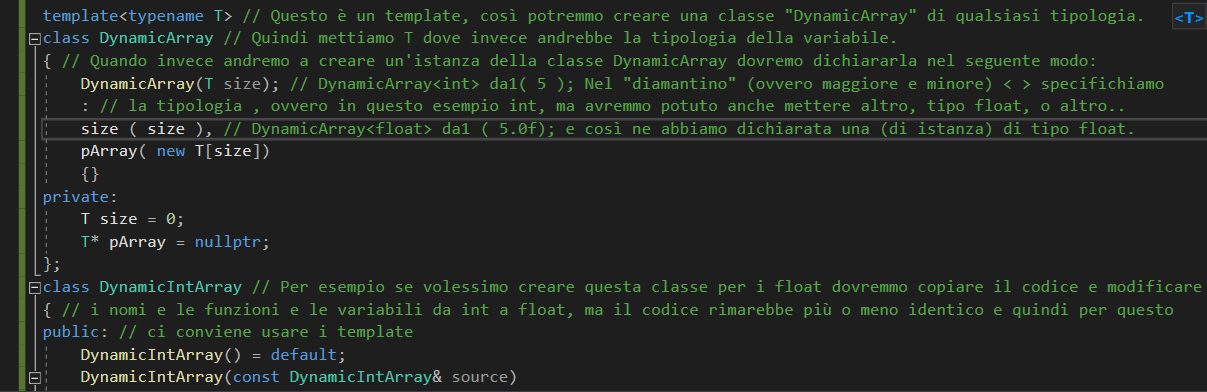
\includegraphics[width=1.2\textwidth, height=1.2\textheight, keepaspectratio]{./imgs/template.png}
	\caption{Template}
	\label{fig:template}
\end{figure}

%TODO: typename

% -------------------------- SECTION: VECTOR -----------------------------------------

%TODO: emplace_back

\section{std::vector<>}

\textsf{\small \textbf{Definizione:} I \textbf{vectors} sono un contenitore rappresentante una array che può cambiare in size (spazio). Sono degli array dinamici.} \\

\textsf{\small I vectors memorizzano i dati in locazioni contigue di memoria e permettono l'accesso diretto a qualsiasi elemento usando l'operatore []. Supportano la riduzione e l'ampiamento dello spazio a runtime (ovvero eseguite mentre il tuo programma è in esecuzione).} \\

\textsf{\small La classe vector fa uso dei template così che possiamo eseguirla con qualsiasi tipo. Per poterla usare avremo bisogno di importare \textbf{\#include <vector>}.} \\

\begin{lstlisting}
	#include <iostream>
	#include <vector>
	
	std::vector<int> v{ 1, 3, 7, 8};
	std::vector<int> v2 = v; // Oppure potevamo scrivere std::vector<int> v2(v);
	
	v2.push_back(9); // Aggiungiamo un elemento.
	
	std::cout << "v size: " << v.size() << std::endl; //Output: v size: 4
	std::cout << "v2 size: " << v2.size() << std::endl; //Output: v2 size: 5
\end{lstlisting}

\textsf{\small Inoltre, la classe vector mette a disposizione tante altre funzioni per la loro manipolazione.} \\

\textsf{\small P.S.: Da non confondere con i vettori in matematica|fisica.} \break

% -------------------------- SECTION: VIRTUAL ----------------------------------------

\newpage

\section{Virtual}

\textsf{\small \textbf{Definizione:} } \\

\subsection{Virtual Inheritance}

\textsf{\small \textbf{Definizione:} } \\

% -------------------------- SECTION: TIPI DI CAST -----------------------------------

%TODO: Prima di spiegare questi dovrei spiegare i templates, altrimenti uno non capisce i <>.
%TODO: Inoltre dovrei parlare anche della keyword virtual e virtual inheritance.

\newpage

\section{Tipi di Casts}

\textsf{\small \textbf{Definizione:} Il \textbf{casting} è un'operazione che permette la conversione di un valore in un altro. In C++ ci sono diversi tipi di casting: } \\

\subsection{static\_cast<>}

\begin{itemize}
	\item \textsf{\small \textbf{static\_cast<> :} Quello che fa è un cast implicito tra tipi (come int a float, o puntatore a void*) e può anche chiamare funzioni esplicite per la conversione. }
\end{itemize}

\begin{lstlisting}
	float f = 3.69;
	int x = static_cast<int>(f);
	std::cout << "x: " << x << std::endl; // Output: x: 3 
\end{lstlisting}

\subsection{const\_cast<>}

\begin{itemize}
	\item \textsf{\small \textbf{const\_cast<> :} Serve per aggiungere o rimuovere il \textbf{const} ad una variabile. Se la variabile che stiamo cercando di modificare era già const allora questo produce un valore indefinito. Se lo si usa per qualcosa che non era dichiarato come const allora è safe (sicuro farlo, non ci saranno problemi).  }
\end{itemize}

\begin{lstlisting}
	#include <iostream>
	
	void print( char* str)
	{
		std::cout << str << '\n';
	}

	int main()
	{
		const char* c = "testo";
		// Ci serve per poter passare un puntatore a char const ad una funzione che prende un puntatore a char senza const.
		print(const_cast<char*>(c)); // Output: testo
		return 0;
	}
\end{lstlisting}

\subsection{dynamic\_cast<>}

\begin{itemize}
	\item \textsf{\small \textbf{dynamic\_cast<> :} Serve esclusivamente per i casts riguardanti il polimorfismo. Puoi castare un puntatore o una reference a qualsiasi altro tipo di classe. Non solo si può fare un casting verso il basso, ma anche in alto e a lato. Il dynamic\_cast cercherà di ritorna l'oggetto desiderato se possibile, altrimenti ritornerà \textbf{nullptr} in caso di un puntatore e \textbf{std::bad\_cast} nel caso di una reference.}
	\item \textsf{\small Ha delle limitazioni. Non funzionerà nel caso in cui diversi oggetti ereditano tutti dallo stessa classe. (il famoso problema del \emph{dreaded diamond}.) e non stai usando l'ereditarietà \textbf{virtual}.}
	\item \textsf{\small Inoltre può soltanto funzionare con l'ereditarietà pubblica, fallirà con l'ereditarietà \textbf{protected} o \textbf{private}. Comunque questi tipi di ereditarietà sono rare.}
\end{itemize}

\begin{lstlisting}
	// C++ programma per dimostrare che se non c'è
	// alcuna funzione virtuale nella Base classe.
	#include <iostream>
	
	// Base class declaration
	class Base {
		void print()
		{
			std::cout << "Base" << std::endl;
		}
	};
	
	// Derived Class 1 declaration
	class Derived1 : public Base {
		void print()
		{
			std::cout << "Derived1" << std::endl;
		}
	};
	
	// Derived class 2 declaration
	class Derived2 : public Base {
		void print()
		{
			std::cout << "Derived2" << std::endl;
		}
	};
	
	// Driver Code
	int main()
	{
		Derived1 d1;
		
		// Base class pointer hold Derived1
		// class object
		Base* bp = dynamic_cast<Base*>(&d1);
		
		// Dynamic casting
		Derived2* dp2 = dynamic_cast<Derived2*>(bp);
		if (dp2 == nullptr)
			std::cout << "null" << std::endl;
			
		// Output: null, in realtà errore.
		return 0;
	}
\end{lstlisting}

\subsection{reinterpret\_cast<>}

\begin{itemize}
	\item \textsf{\small \textbf{reinterpret\_cast<> :} È quello più pericoloso di tutti e quindi bisogna utilizzarlo con moderazione. Trasforma un tipo direttamente in un altro come cast da un puntatore ad un altro o memorizzare un puntatore in un int, ecc..}
	\item \textsf{\small L'unica cosa garantita con questo tipo di cast è che se torni indietro al tipo originale riotterrai lo stesso valore (non succederà se il tipo era più piccolo del tipo originale.)}
\end{itemize}

\begin{lstlisting}
	class A {
		public:
			int x;
	};

	class B {
		public:
			int x;
	};

	A *a = new A;
	B *b = reinterpret_cast<*B>(a);
	
	a->x = 5;
	std::cout << "b: " << b->x << std::endl; // Output: b: 5
	std::cout << "a: " << a->x << std::endl; // Output: a: 5
\end{lstlisting}

\subsection{C-style \& function-style cast o Regular Cast}

\begin{itemize}
	\item \textsf{\small Questo tipo di cast chiamato \textbf{Regular Cast} o \textbf{C-style cast} (derivando dal C ovviamente) è molto più potente degli altri tipi di cast, ma allo stesso tempo molto meno sicuro.}
	\item \textsf{\small Ignorano i controlli d'accesso quando si esegue uno static\_cast.}
	\item \textsf{\small Permette di fare un cast sicuro ad una classe privata, mentre il suo "equivalente" static\_cast darebbe un errore a tempo di compilazione (compile-time).}
\end{itemize}

\begin{lstlisting}
	double d = 9.87;
	int x;
	
	x = (int)d;
	std::cout << "x: " << x std::endl; // Output: x: 9
\end{lstlisting}

\subsection{Ricapitolando}

\begin{tabular}{|c|c|}
	\hline
	\textbf{Cast} & \textbf{Definizione} \\
	\hline
	\textbf{dynamic\_cast} & \textsf{\small per convertire puntatori/references in una gerarchia di ereditarietà.} \\
	\hline
	\textbf{static\_cast} & \textsf{\small per le conversioni di tipi ordinari.} \\
	\hline
	\textbf{reinterpret\_cast} & \textsf{\small per reinterpretare bit patterns di basso livello. Usare con cauzione.} \\
	\hline
	\textbf{const\_cast} & \textsf{\small per aggiungere/rimuovere \textbf{const} al cast.} \\
	\hline
\end{tabular}

%TODO: typeid

% -------------------------- SECTION: LAMBDAS ----------------------------------------

\section{Lambdas}

\textsf{\small \textbf{Definizione:} } \\

% -------------------------- SECTION: MEMORIA DINAMICA -------------------------------

%TOOD: memoria dinamica, new, delete, ecc..

% -------------------------- SECTION: TIPI DI COSTRUTTORI | RULE OF 3 ----------------

% -------------------------- SECTION: RULE OF 5 --------------------------------------

% -------------------------- SECTION: RAII -------------------------------------------

% -------------------------- SECTION: CLASSI ASTRATTE --------------------------------

% -------------------------- SECTION: ITERATORI --------------------------------------

% -------------------------- SECTION: ECCEZIONI --------------------------------------

%TODO: try/catch
%TODO: Errori a compile-time ed errori a runtime.
%TODO: throw.
%TODO: std::throw exception

% -------------------------- SECTION: OPERAZIONI SU FILE -----------------------------

%TODO: numeri pseudo-random?
%TODO: std::chrono

% -------------------------- SECTION: MOVE SEMANTICS ---------------------------------